\documentclass{article}
\usepackage[a4paper, total={6.6in, 9in}]{geometry}
\usepackage{amsmath}
\usepackage{amssymb}
\usepackage{authblk}
\usepackage{bbm}
\usepackage{booktabs}
\usepackage{diagbox}
\usepackage{graphicx}
\usepackage{listings}
\usepackage{multirow}
\usepackage{xcolor}
\usepackage[colorlinks=true,
    linkcolor=blue, 
    urlcolor=blue, 
    citecolor=blue, 
    anchorcolor=blue]{hyperref}
%\usepackage{slashbox}
\allowdisplaybreaks

\title{CSCI-SHU 360 Machine Learning\\
    Report of Final Competition}
\author{Yufeng \textsc{-AeoLian-} Xu  \texttt{yx3038@nyu.edu}}

\begin{document}
    \maketitle

    \section{Guideline}
    This section aims to provide a navigation of this repository. 
    \begin{itemize}
        \item Folder \textbf{src} contains the source code of the final competition.
        \item File \textbf{main.py} is the main file for training of the models. File \textbf{data\_utils.py} contains the functions for data processing as well as the customized dataset class. File \textbf{models.py} contains the customized ResNet18. File \textbf{infer.py} utilizes the ensemble of several trained model to make predictions.
        \item Folder \textbf{write-up} contains the report on the final competition.
        \item Folder \textbf{checkpoints} records the parameters, prediction, as well as best validation accurcay so far for each of the models.
        \item Folder \textbf{data} contains the original as well as processed data.
        \item File \textbf{prediction.csv} is the prediction made by \textbf{infer.py}.
    \end{itemize}

    \section{Data Preprocessing}
    We called a Python library called \textbf{spleeter} to separate vocal and instrumental parts in each music snippet, and chose and vocal parts as our training and evaluation  data. Afterwards, we used \textbf{torchaudio} to load and transform(or augment) the vocal files.

    \section{Models}
    The models I have tried for the final competition include: ResNet18, ResNet50, ResNet101, ResNext, DenseNet201, Vision Transformer (ViT), Long Short Term Memory (LSTM).
    Among all these models, ResNet18 demonstrates excellent performance and the best performance-efficiency tradeoff. Therefore, the final results are based on resnet18. An unexpected observation is that the resnet18 network implemented by myself has better performance than the built-in one from torch, although according to \textbf{model.modules} the two have exactly the same components.

    \section{Training Setups}
    \subsection*{Vocal Separation}
    \begin{figure}[hbt!]
        \centering
        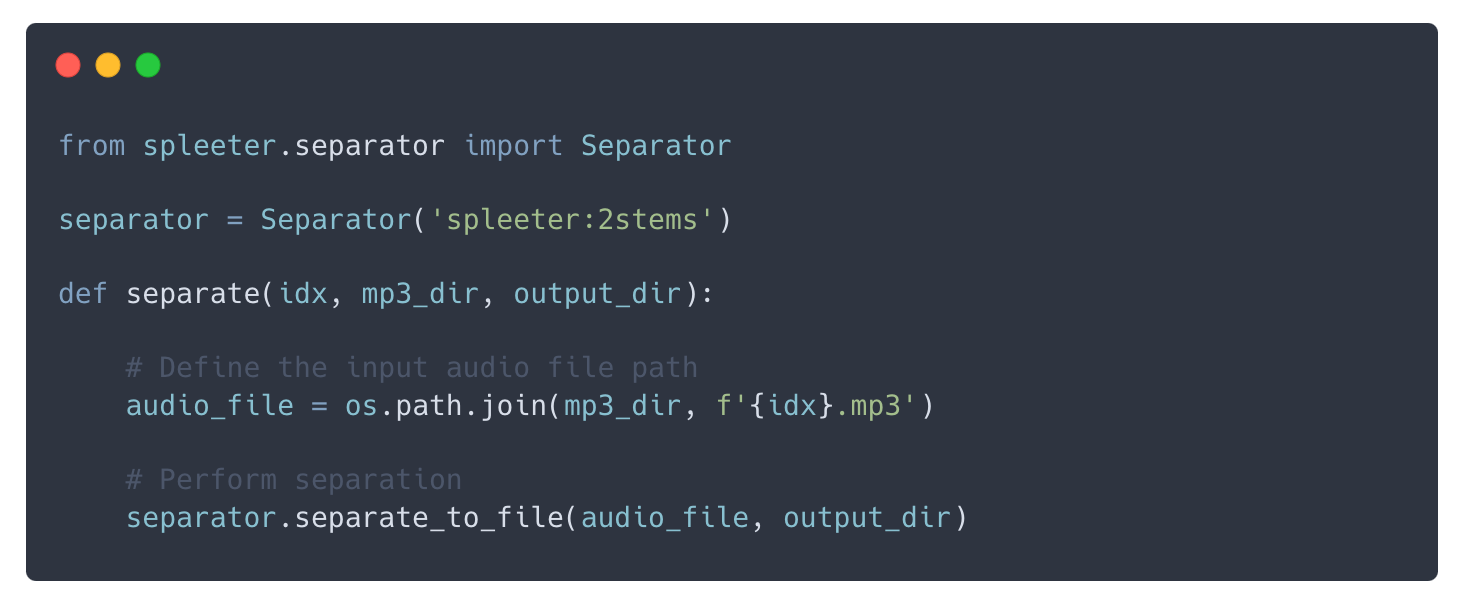
\includegraphics[width=0.8\textwidth]{figs/separate.png}
    \end{figure}
    \subsection*{Data Transformatation}
    \begin{figure}[hbt!]
        \centering
        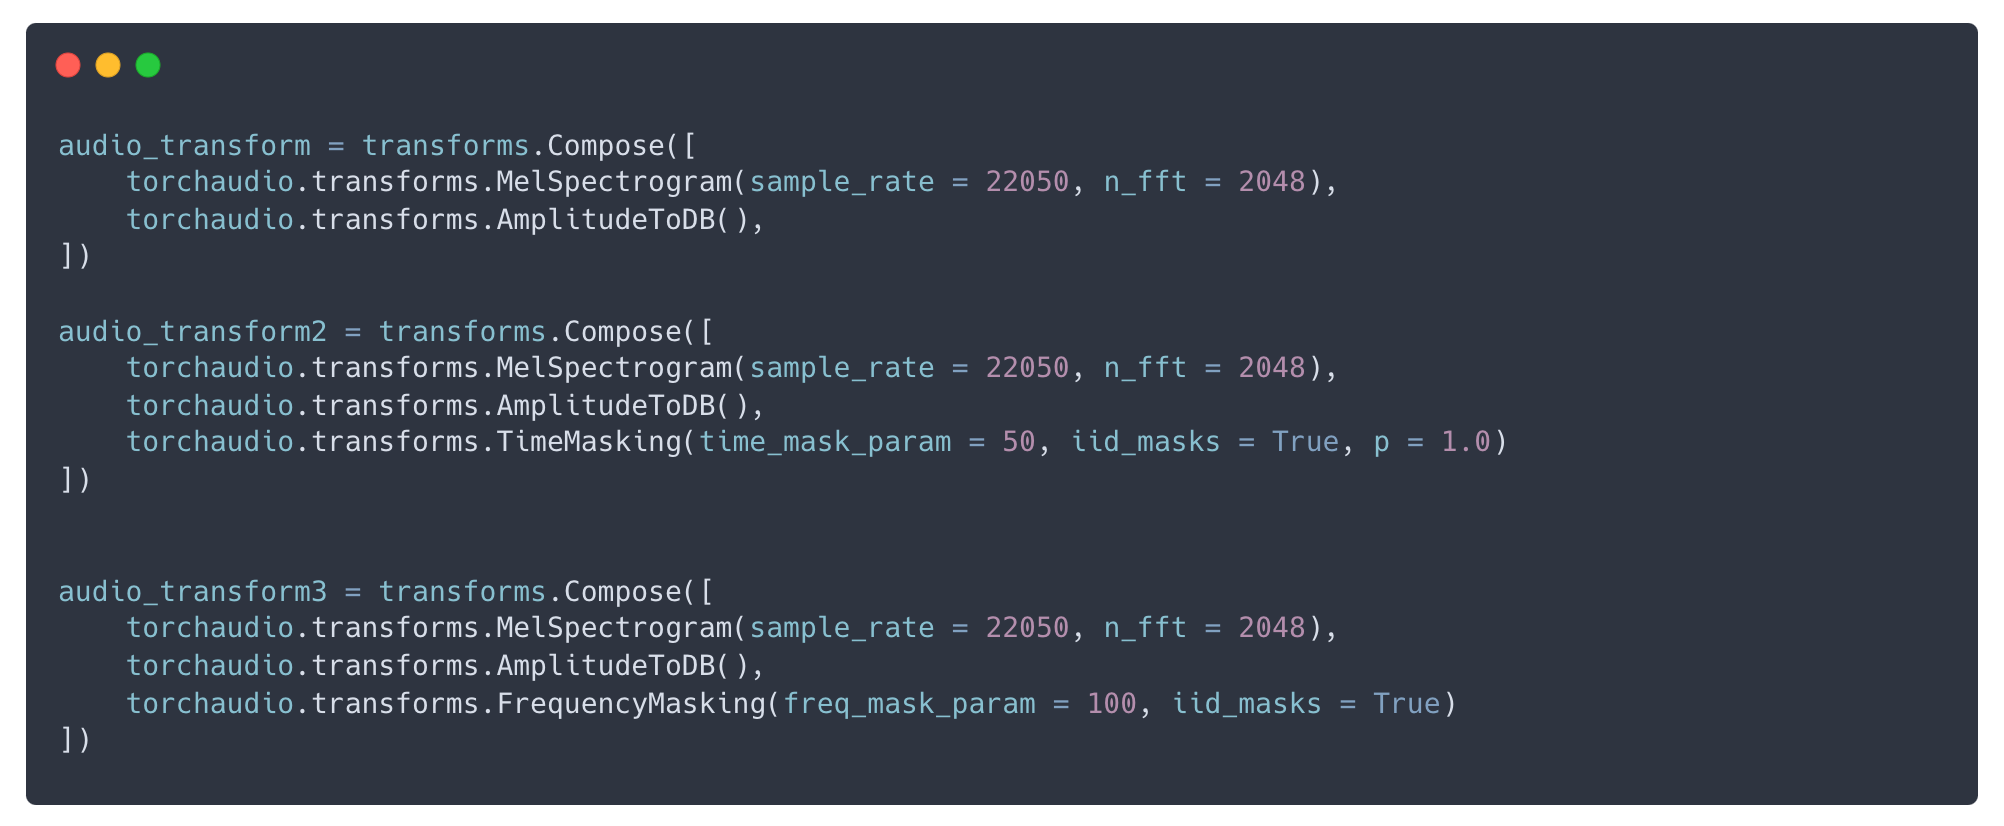
\includegraphics[width=1.0\textwidth]{figs/augment.png}
    \end{figure}
    \subsection*{Optimization}
    \begin{figure}[hbt!]
        \centering
        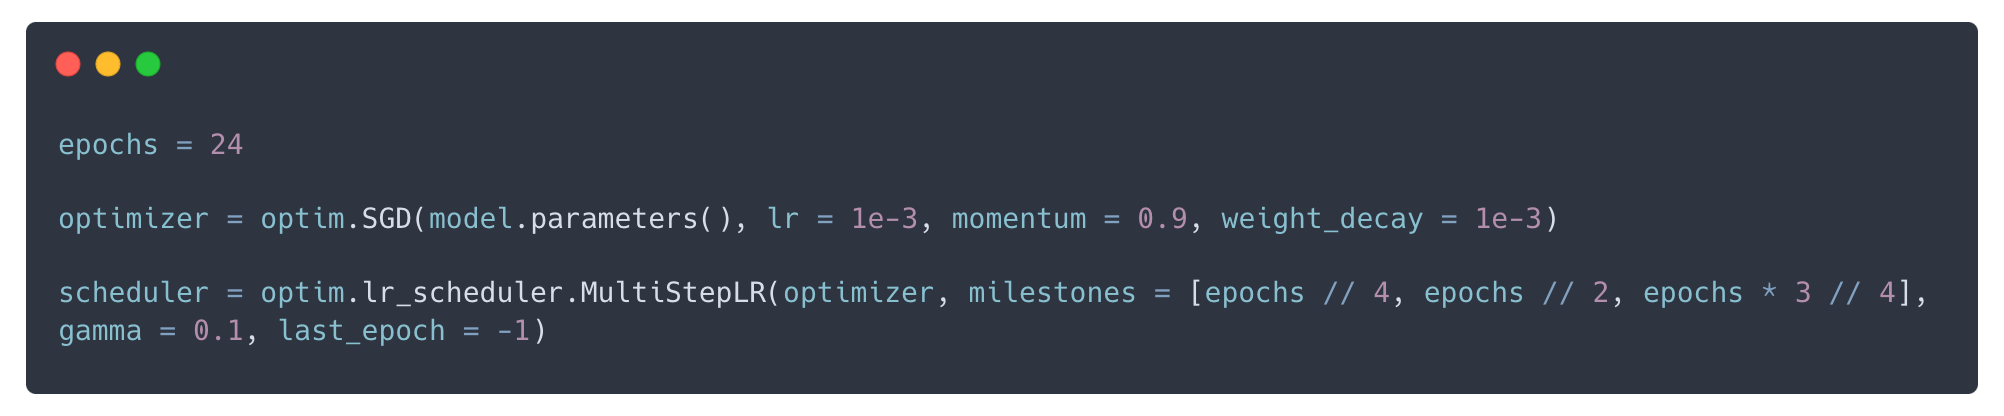
\includegraphics[width=1.0\textwidth]{figs/optimization.png}
    \end{figure}

    \section{Discussion}



\end{document}